\documentclass[../main.tex]{subfiles}

\begin{document}
A \textbf{function} $f$ on a set $D$ into a set $R$ is a rule that assigns a unique element $f(x)$ in $R$ to each element $x$ in $D$.

$D$ is called the \textbf{domain} of $f$. $R$ is called the target or \textbf{codomain} of $f$. The \textbf{range} of $f$ is a subset of $R$ containing of all possible values $f(x)$.

\textit{
This definition is not mathematical as we did not define what a rule is. Formally one defines a function as a relation.}

\begin{figure}[H]
  \centering
  \subfloat[a]{
  \scalebox{.8}{\begin{tikzpicture}
  %put some nodes on the left
  \foreach \x in {1,2,3}{
  \node[fill,circle,inner sep=2pt] (d\x) at (0,\x) {};
  }
  \node (D) at (-0.5,4) {D};
  \node[fit=(d1) (d2) (d3),ellipse,draw,minimum width=1cm] {};
  %put some nodes on the center
  \foreach \x[count=\xi] in {0.5,1.5,...,4}{
  \node[fill,circle,inner sep=2pt] (r\xi) at (2,\x) {};
  }
  \node (S) at (2.8,4) {R};
  \node[fit=(r1) (r2) (r3) (r4),ellipse,draw,minimum width=1.5cm] {};
  \draw[-latex] (d1) -- (r2);
  \draw[-latex] (d2) -- (r2);
  \draw[-latex] (d3) -- (r4);
  \draw[-latex] (d3) -- (r4);
\end{tikzpicture}}
  }
  \subfloat[b]{
  \scalebox{.8}{\begin{tikzpicture}
%put some nodes on the left
\foreach \x in {1,2,3}{
\node[fill,circle,inner sep=2pt] (d\x) at (0,\x) {};
}
\node (D) at (-0.5,4) {D};
\node[fit=(d1) (d2) (d3),ellipse,draw,minimum width=1cm] {};
%put some nodes on the center
\foreach \x[count=\xi] in {0.5,1.5,...,4}{
\node[fill,circle,inner sep=2pt] (r\xi) at (2,\x) {};
}
\node (S) at (2.8,4) {R};
\node[fit=(r1) (r2) (r3) (r4),ellipse,draw,minimum width=1.5cm] {};
\draw[-latex] (d1) -- (r1);
\draw[-latex] (d2) -- (r2);
\draw[-latex] (d2) -- (r3);
\draw[-latex] (d3) -- (r4);
\end{tikzpicture}}
  }
  \caption{a) Not a function. b) A Function }
  \label{fig:funcNotfunc}
\end{figure}

\begin{example}
  Define a function on the set of all real numbers by $f(x)=x^2+1$. Find $f(0), \, f(2), \, f(x+2)$.
\end{example}

\[
  f(x) = \frac{1}{x}, \qquad x > 0
\]
means that the domain of $f$ is the set $\{x \mid x > 0\}$.

Technically, this function is different from the function
\[
  f(x) = \frac{1}{x}, \qquad x < 0.
\]

If we do not specify the domain of a function $f$, then the \textbf{domain convention} is to assume that the domain of $f$ is the set of all real numbers for which $f$ is defined.

So if we write
\[
  f(x)=\frac{1}{x},
\]
we are assuming $f$ is defined for all real numbers except $0$.


\begin{example}
  Find the domain of $f(x) = \sqrt{2-x}$.

  \textbf{Solution.} Its domain is all $x$ for which $2-x \ge 0$, i.e. the interval $(-\infty, 2]$.
\end{example}

\begin{example}
    Find the domain of $f(x) = \frac{1}{x^2 - x}$.
\end{example}

A function $f: D \to R$ is \textbf{1-1} if $f(x_1) = f(x_2)$ then $x_1=x_2$. A function $f: D \to R$ is \textbf{onto} if for every $y \in R$, there is an $x \in D$ such that $f(x) = y$.

\begin{example}
  Draw functions which are 1-1, onto, not 1-1 and not onto,  similar to the Figure~\ref{fig:funcNotfunc}.
\end{example}

\subsection*{Graph of a function}
The \emph{graph of a function} $f$ is the set of all points whose coordinates are $(x, f(x))$ where $x$ is in the domain of $f$.

\begin{figure}[th]
  \centering
  
\begin{picture} (240.000000,144.800000)(0,0)
\put(0.0, 0.0){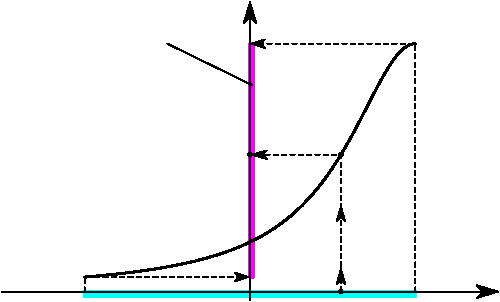
\includegraphics{figures/P4-graphOFf.pdf}}
    \put( 80.33, 123.97){\sffamily\itshape \makebox[0pt][r]{range of $f$}}
    \put(118.00,  70.71){\sffamily\itshape \makebox[0pt][r]{$y=f(x)$}}
    \put(167.63,  68.71){\sffamily\itshape $(x, f(x))$}
    \put(167.63,   6.97){\sffamily\itshape $x$}
    \put(120.00,  -7.03){\sffamily\itshape \makebox[0pt][c]{domain of $f$}}
\end{picture}

\end{figure}



\begin{example}
  A function which is given by the formula
  \[
    f(x) = mx + n
  \]
  where $m$ and $n$ are constants is called a \emph{linear function}. Its graph is a straight line. The constants $m$ and $n$ are the \emph{slope} and \emph{$y$-intercept} of the line.
\end{example}

\begin{example}
  The square root function $f(x) = \sqrt{x}$ has domain $[0, \infty)$ and takes $x$ to its positive square root. Hence it has range $[0, \infty)$.
\end{example}

\begin{example}
  The absolute value function $f(x) = \abs{x} = \sqrt{x^2}$ has domain $(-\infty, \infty)$ and range $[0, \infty)$.
\end{example}

\begin{example}
  Draw the graphs of some elementary functions
  \[
    c, x, x^2, \sqrt{x}, x^3, x^{1/3}, \frac{1}{x}, \frac{1}{x^2}, \sqrt{1-x^2}, \abs{x}.
  \]
\end{example}
\begin{example}
  Sketch the graph of $f(x)=1+\sqrt{x-4}$.

  Solution: Shift the graph of $y=\sqrt{x}$ 1 unit up and 4 units to the right.
\end{example}
\begin{example}
  Sketch the graph of the function $f(x) = \frac{2-x}{x-1}$.

  Solution. $f(x) = \frac{2-x}{x-1} = -1 + \frac{1}{x-1}$. So shift the graph of $y=\frac{1}{x}$ 1 unit down and 1 unit to the right.
\end{example}

\subsection*{Vertical Line Test}
\emph{The graph of a function cannot intersect a vertical line ``$x=\text{\em constant}$'' in more than one point}.

For example, the circle $x^2+y^2=1$ is not a graph of a function.
\begin{figure}[H]
  \centering
  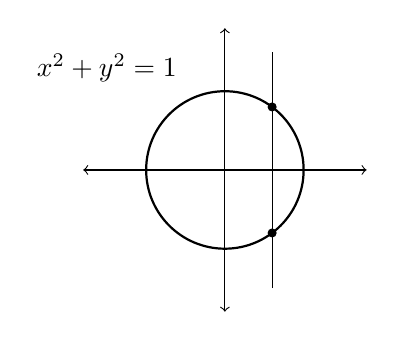
\begin{tikzpicture}
  \draw[<->] (-1.8,0) -- (1.8,0);
  \draw[<->] (0,-1.8) -- (0,1.8);
  \draw[thick] (0,0) circle [radius=1];
  \draw[] (0.6, -1.5) -- (0.6, 1.5);
  \draw[fill, black] (0.6, 0.8) circle [radius=0.05];
  \draw[fill, black] (0.6, -0.8) circle [radius=0.05];
  \node[] at (-1.5, 1.3) {$x^2+y^2=1$};
\end{tikzpicture}
\end{figure}

\subsection*{Even and Odd Functions}

\begin{definition}
We say that $f$ is an \textbf{even function} if $f\left( -x\right) =f\left( x\right) $ for every $x\in D$.
We say that $f$ is an \textbf{odd function} if $f(-x)=-f(x)$ for every $x\in D$.
\end{definition}

\begin{figure}[H]
  \centering
  \subfloat[a]{
  \begin{tikzpicture}[scale=2]
  \draw [<->] (-1,0) -- (1,0);
  \draw [<->] (0,-1) -- (0,1);
  \node[below] (X1) at (0.7, 0) {$x$};
  \node[below] (X2) at (-0.7, 0) {$-x$};
  \draw[domain=-1:1] plot (\x, {\x*\x+0.1});
  \draw[dashed] (X1)--(0.7, 0.59);
  \draw[dashed] (X2)--(-0.7, 0.59);
  \draw[dashed] (0.7, 0.59)--(-0.7, 0.59);
  \node[above left] (fx) at (0, 0.59) {$f(x)$};
  \draw[fill] (0, 0.59) circle [radius=.025];
\end{tikzpicture}
  }
  \subfloat[b]{
  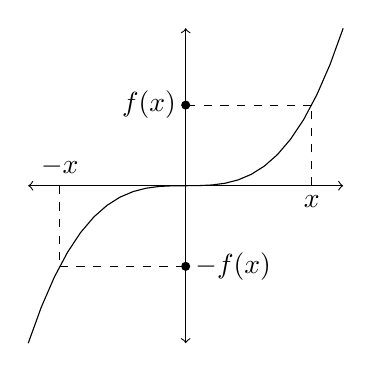
\begin{tikzpicture}[scale=2]
  \draw [<->] (-1,0) -- (1,0);
  \draw [<->] (0,-1) -- (0,1);
  \node[below] (X1) at (0.8, 0) {$x$};
  \node[above] (X2) at (-0.8, 0) {$-x$};
  \draw[domain=-1:1] plot (\x, {\x*\x*\x});
  \draw[dashed] (X1)--(0.8, 0.512);
  \draw[dashed] (X2)--(-0.8, -0.512);
  \draw[dashed] (0.8, 0.512)--(0, 0.512);
  \draw[dashed] (-0.8, -0.512)--(0, -0.512);
  \node[left] at (0, 0.512) {$f(x)$};
  \draw[fill] (0, 0.512) circle [radius=.025];
  \node[right] at (0, -0.512) {$-f(x)$};
  \draw[fill] (0, -0.512) circle [radius=.025];
\end{tikzpicture}
  }
  \caption{a) An even function,  b) An odd function.}
\end{figure}

Odd functions are symmetric with respect to origin and even functions are symmetric with respect to the $y$-axis.


\begin{example}
$f(x)=x,f(x)=x^{3}$ are odd and $f(x)=x^{2}$ and $f(x) =x^{4}$ are even and $f(x)=\frac{1}{x+1}$ is neither even or odd.
\end{example}

\begin{example}
$f(x)=x^{3}+x$ is odd and $f(x)=\frac{1}{x^{2}-1}$ is even and $f(x)=x^{2}+x$
is either even or odd.
\end{example}

\end{document}